\documentclass{ximera}
\usetikzlibrary{arrows.meta}
\usepackage{draftwatermark}
\SetWatermarkScale{2}
\SetWatermarkLightness{0.9}
\SetWatermarkText{\textsf{\shortstack{DRAFT  \\[0.5cm] {\fontsize{38}{12}\selectfont \today}}}}

\newcommand{\recommendation}[1]{\textbf{(Recommended by #1)}}

\newcommand{\BADBAD}{\marginpar{\textbf{BADBAD}}}

\begin{document}
\begin{abstract}
\end{abstract}

\section{Number line questions}

\begin{problem}
  Two real numbers, $x$ and $y$, are shown below on a number line.
  \begin{image}
  \begin{tikzpicture}[x=0.15\textwidth]
    \draw[-{>[scale=1.75]}] (-0.05\textwidth,0) -- (0.8\textwidth,0);
    \foreach \x in {0,...,5} {%
      \draw (\x,-.1) -- (\x,.1);
      \node[anchor=north,yshift=-2pt] at (\x,0) {$\x$};
    }
    \draw (1.25,0) node [circle,fill,inner sep=1pt,label=above:$x$](e){};
    \draw (2.16,0) node [circle,fill,inner sep=1pt,label=above:$y$](e){};
  \end{tikzpicture}
  \end{image}
  What is the best guess for $xy$?
  \begin{multipleChoice}
    \choice{1.1}
    \choice[correct]{2.7}
    \choice{4.2}
    \choice{6.5}
  \end{multipleChoice}
\end{problem}

\begin{problem}
  Two real numbers, $x$ and $y$, are shown below on a number line.
  \begin{image}
  \begin{tikzpicture}[x=0.16\textwidth]
    \draw[-{>[scale=1.75]}] (-0.05\textwidth,0) -- (0.8\textwidth,0);
    \foreach \x in {0,...,4} {%
      \draw (\x,-.1) -- (\x,.1);
      \node[anchor=north,yshift=-2pt] at (\x,0) {$\x$};
    }
    \draw (0.85,0) node [circle,fill,inner sep=1pt,label=above:$x$](e){};
    \draw (3.40,0) node [circle,fill,inner sep=1pt,label=above:$y$](e){};
  \end{tikzpicture}
  \end{image}
  What is the best guess for $y/x$?
  \begin{multipleChoice}
    \choice{2.89}
    \choice{3}
    \choice[correct]{4}
    \choice{6}
  \end{multipleChoice}
\end{problem}

\begin{problem}
  Four numbers $A$, $B$, $C$, and $D$ are shown below on a number line.
  \begin{image}
  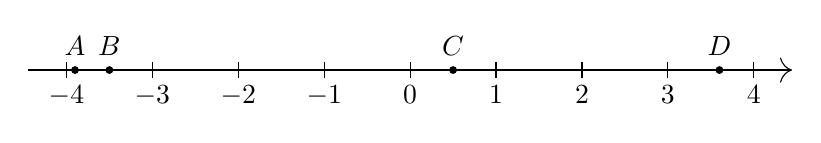
\begin{tikzpicture}[x=0.09\textwidth]
    \draw[-{>[scale=1.75]}] (-0.4\textwidth,0) -- (0.4\textwidth,0);
    \foreach \x in {-4,...,4} {%
      \draw (\x,-.1) -- (\x,.1);
      \node[anchor=north,yshift=-2pt] at (\x,0) {$\x$};
    }
    \draw (-3.9,0) node [circle,fill,inner sep=1pt,label=above:$A$](e){};
    \draw (-3.5,0) node [circle,fill,inner sep=1pt,label=above:$B$](e){};
    \draw (0.5,0) node [circle,fill,inner sep=1pt,label=above:$C$](e){};
    \draw (3.6,0) node [circle,fill,inner sep=1pt,label=above:$D$](e){};
  \end{tikzpicture}
  \end{image}
  Which is closest to the average of $A$, $B$, $C$, $D$?
  \begin{multipleChoice}
    \choice{$A$}
    \choice{$B$}
    \choice[correct]{$C$}
    \choice{$D$}
  \end{multipleChoice}
\end{problem}


\begin{problem}
  Two numbers, $x$ and $y$, are shown below on a number line.
  \begin{image}
    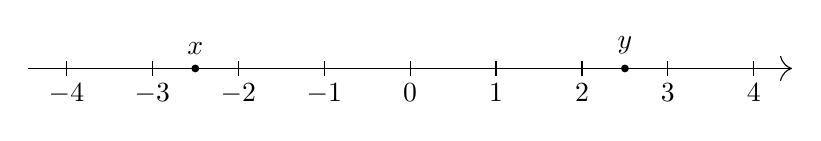
\begin{tikzpicture}[x=0.09\textwidth]
      \draw[-{>[scale=1.75]}] (-0.4\textwidth,0) -- (0.4\textwidth,0);
      \foreach \x in {-4,...,4} {%
        \draw (\x,-.1) -- (\x,.1);
        \node[anchor=north,yshift=-2pt] at (\x,0) {$\x$};
      }
      \draw (-2.5,0) node [circle,fill,inner sep=1pt,label=above:$x$](e){};
      \draw (2.5,0) node [circle,fill,inner sep=1pt,label=above:$y$](e){};
    \end{tikzpicture}
  \end{image}
  Which is closest to $xy$?
  \begin{multipleChoice}
    \choice[correct]{$-6.25$}
    \choice{$-4.75$}
    \choice{$4.75$}
    \choice{$6.25$}
  \end{multipleChoice}
\end{problem}


\begin{problem}
  Two numbers, $x$ and $y$, are shown below on a number line.
  \begin{image}
    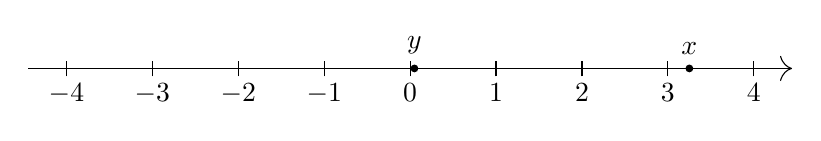
\begin{tikzpicture}[x=0.09\textwidth]
      \draw[-{>[scale=1.75]}] (-0.4\textwidth,0) -- (0.4\textwidth,0);
      \foreach \x in {-4,...,4} {%
        \draw (\x,-.1) -- (\x,.1);
        \node[anchor=north,yshift=-2pt] at (\x,0) {$\x$};
      }
      \draw (3.25,0) node [circle,fill,inner sep=1pt,label=above:$x$](e){};
      \draw (0.05,0) node [circle,fill,inner sep=1pt,label=above:$y$](e){};
    \end{tikzpicture}
  \end{image}
  What can be said about $x/y$?
  \begin{multipleChoice}
    \choice{$x/y$ is very negative}
    \choice{$x/y$ is close to zero}
    \choice[correct]{$x/y$ is large and positive}
  \end{multipleChoice}
\end{problem}

\begin{problem}
  Two numbers, $x$ and $y$, are shown below on a number line.
  \begin{image}
    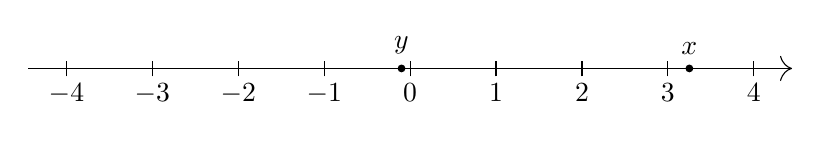
\begin{tikzpicture}[x=0.09\textwidth]
      \draw[-{>[scale=1.75]}] (-0.4\textwidth,0) -- (0.4\textwidth,0);
      \foreach \x in {-4,...,4} {%
        \draw (\x,-.1) -- (\x,.1);
        \node[anchor=north,yshift=-2pt] at (\x,0) {$\x$};
      }
      \draw (3.25,0) node [circle,fill,inner sep=1pt,label=above:$x$](e){};
      \draw (-0.1,0) node [circle,fill,inner sep=1pt,label=above:$y$](e){};
    \end{tikzpicture}
  \end{image}
  What can be said about $x/y$?
  \begin{multipleChoice}
    \choice[correct]{$x/y$ is very negative}
    \choice{$x/y$ is close to zero}
    \choice{$x/y$ is large and positive}
  \end{multipleChoice}
\end{problem}

\begin{problem}
  The number $x$ is shown below on a number line.
  \begin{image}
    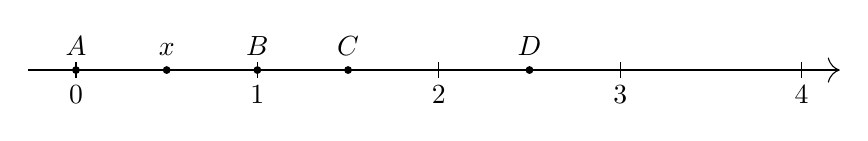
\begin{tikzpicture}[x=0.19\textwidth]
      \draw[-{>[scale=1.75]}] (-0.05\textwidth,0) -- (0.8\textwidth,0);
      \foreach \x in {0,...,4} {%
        \draw (\x,-.1) -- (\x,.1);
        \node[anchor=north,yshift=-2pt] at (\x,0) {$\x$};
      }
      \draw (0.5,0) node [circle,fill,inner sep=1pt,label=above:$x$](e){};
      \draw (0,0) node [circle,fill,inner sep=1pt,label=above:$A$](e){};
      \draw (1,0) node [circle,fill,inner sep=1pt,label=above:$B$](e){};
      \draw (1.5,0) node [circle,fill,inner sep=1pt,label=above:$C$](e){};
      \draw (2.5,0) node [circle,fill,inner sep=1pt,label=above:$D$](e){};
    \end{tikzpicture}
  \end{image}
  Which number is closer to $\sqrt{x}$?
  \begin{multipleChoice}
    \choice{$A$}
    \choice[correct]{$B$}
    \choice{$C$}
    \choice{$D$}
  \end{multipleChoice}
\end{problem}

\begin{problem}
  The number $x$ is shown below on a number line.
  \begin{image}
    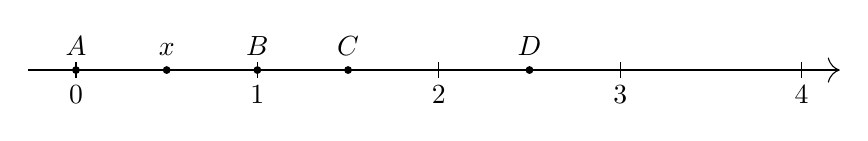
\begin{tikzpicture}[x=0.19\textwidth]
      \draw[-{>[scale=1.75]}] (-0.05\textwidth,0) -- (0.8\textwidth,0);
      \foreach \x in {0,...,4} {%
        \draw (\x,-.1) -- (\x,.1);
        \node[anchor=north,yshift=-2pt] at (\x,0) {$\x$};
      }
      \draw (0.5,0) node [circle,fill,inner sep=1pt,label=above:$x$](e){};
      \draw (0,0) node [circle,fill,inner sep=1pt,label=above:$A$](e){};
      \draw (1,0) node [circle,fill,inner sep=1pt,label=above:$B$](e){};
      \draw (1.5,0) node [circle,fill,inner sep=1pt,label=above:$C$](e){};
      \draw (2.5,0) node [circle,fill,inner sep=1pt,label=above:$D$](e){};
    \end{tikzpicture}
  \end{image}
  Which number is closer to $x^2$?
  \begin{multipleChoice}
    \choice[correct]{$A$}
    \choice{$B$}
    \choice{$C$}
    \choice{$D$}
  \end{multipleChoice}
\end{problem}

\begin{problem}
  Four equally spaced numbers are shown below on a number line.
  \begin{image}
    \begin{tikzpicture}[x=0.19\textwidth]
      \draw[-{>[scale=1.75]}] (-0.05\textwidth,0) -- (0.8\textwidth,0);
      \foreach \x in {0,...,4} {%
        \draw (\x,-.1) -- (\x,.1);
        \node[anchor=north,yshift=-2pt] at (\x,0) {$\x$};
      }
      \draw (0.5,0) node [circle,fill,inner sep=1pt,label=above:$a$](e){};
      \draw (1.5,0) node [circle,fill,inner sep=1pt,label=above:$b$](e){};
      \draw (2.5,0) node [circle,fill,inner sep=1pt,label=above:$c$](e){};
      \draw (3.5,0) node [circle,fill,inner sep=1pt,label=above:$d$](e){};
    \end{tikzpicture}
  \end{image}
  Let $f(x) = \ln x$ and consider $f(a)$ and $f(b)$ and $f(c)$ and $f(d)$.  Which pair of numbers is farthest apart?
  \begin{multipleChoice}
    \choice[correct]{$f(a)$ and $f(b)$}
    \choice{$f(b)$ and $f(c)$}
    \choice{$f(c)$ and $f(d)$}
    \choice{These pairs are all equally far apart}
  \end{multipleChoice}
\end{problem}

\begin{problem}
  Four equally spaced numbers are shown below on a number line.
  \begin{image}
    \begin{tikzpicture}[x=0.19\textwidth]
      \draw[-{>[scale=1.75]}] (-0.05\textwidth,0) -- (0.8\textwidth,0);
      \foreach \x in {0,...,4} {%
        \draw (\x,-.1) -- (\x,.1);
        \node[anchor=north,yshift=-2pt] at (\x,0) {$\x$};
      }
      \draw (0.5,0) node [circle,fill,inner sep=1pt,label=above:$a$](e){};
      \draw (1.5,0) node [circle,fill,inner sep=1pt,label=above:$b$](e){};
      \draw (2.5,0) node [circle,fill,inner sep=1pt,label=above:$c$](e){};
      \draw (3.5,0) node [circle,fill,inner sep=1pt,label=above:$d$](e){};
    \end{tikzpicture}
  \end{image}
  Let $f(x) = x^2$ and consider $f(a)$ and $f(b)$ and $f(c)$ and $f(d)$.  Which pair of numbers is farthest apart?
  \begin{multipleChoice}
    \choice{$f(a)$ and $f(b)$}
    \choice{$f(b)$ and $f(c)$}
    \choice[correct]{$f(c)$ and $f(d)$}
    \choice{These pairs are all equally far apart}
  \end{multipleChoice}
\end{problem}

\begin{problem}
  Two numbers, $s$ and $t$, are shown below.
  \begin{image}
    \begin{tikzpicture}[x=0.19\textwidth]
      \draw[-{>[scale=1.75]}] (-0.05\textwidth,0) -- (0.8\textwidth,0);
      \foreach \x in {0,...,4} {%
        \draw (\x,-.1) -- (\x,.1);
        \node[anchor=north,yshift=-2pt] at (\x,0) {$\x$};
      }
      \draw (2.15,0) node [circle,fill,inner sep=1pt,label=above:$s$](e){};
      \draw (2.45,0) node [circle,fill,inner sep=1pt,label=above:$t$](e){};
    \end{tikzpicture}
  \end{image}
  Let $f(x) = 1/x$.  How does $f(s)$ compare with $f(t)$?
  \begin{multipleChoice}
    \choice{$f(s) < f(t)$}
    \choice{$f(s) = f(t)$}
    \choice[correct]{$f(s) > f(t)$}
  \end{multipleChoice}
\end{problem}

\begin{problem}
  Two pairs of numbers are shown below.
  \begin{image}
    \begin{tikzpicture}[x=0.19\textwidth]
      \draw[-{>[scale=1.75]}] (-0.05\textwidth,0) -- (0.8\textwidth,0);
      \foreach \x in {0,...,4} {%
        \draw (\x,-.1) -- (\x,.1);
        \node[anchor=north,yshift=-2pt] at (\x,0) {$\x$};
      }
      \draw (0.25,0) node [circle,fill,inner sep=1pt,label=above:$s$](e){};
      \draw (1.25,0) node [circle,fill,inner sep=1pt,label=above:$s+h$](e){};
      \draw (2.75,0) node [circle,fill,inner sep=1pt,label=above:$t$](e){};
      \draw (3.75,0) node [circle,fill,inner sep=1pt,label=above:$t+h$](e){};
    \end{tikzpicture}
  \end{image}
  Let $f(x) = x^3$.  How does $f(s+h)-f(s)$ compare with $f(t+h) - f(t)$?
  \begin{multipleChoice}
    \choice[correct]{$f(s+h) - f(s) < f(t+h) - f(t)$}
    \choice{$f(s+h) - f(s) = f(t+h) - f(t)$}
    \choice{$f(s+h) - f(s) > f(t+h) - f(t)$}
  \end{multipleChoice}
\end{problem}

\begin{problem}
  Two pairs of numbers are shown below.
  \begin{image}
    \begin{tikzpicture}[x=0.19\textwidth]
      \draw[-{>[scale=1.75]}] (-0.05\textwidth,0) -- (0.8\textwidth,0);
      \foreach \x in {0,...,4} {%
        \draw (\x,-.1) -- (\x,.1);
        \node[anchor=north,yshift=-2pt] at (\x,0) {$\x$};
      }
      \draw (0.25,0) node [circle,fill,inner sep=1pt,label=above:$s$](e){};
      \draw (1.25,0) node [circle,fill,inner sep=1pt,label=above:$s+h$](e){};
      \draw (2.75,0) node [circle,fill,inner sep=1pt,label=above:$t$](e){};
      \draw (3.75,0) node [circle,fill,inner sep=1pt,label=above:$t+h$](e){};
    \end{tikzpicture}
  \end{image}
  Let $f(x) = -1/x$.  How does $f(s+h)-f(s)$ compare with $f(t+h) - f(t)$?
  \begin{multipleChoice}
    \choice{$f(s+h) - f(s) < f(t+h) - f(t)$}
    \choice{$f(s+h) - f(s) = f(t+h) - f(t)$}
    \choice[correct]{$f(s+h) - f(s) > f(t+h) - f(t)$}
  \end{multipleChoice}
\end{problem}

\begin{problem}
  Two pairs of numbers are shown below.
  \begin{image}
    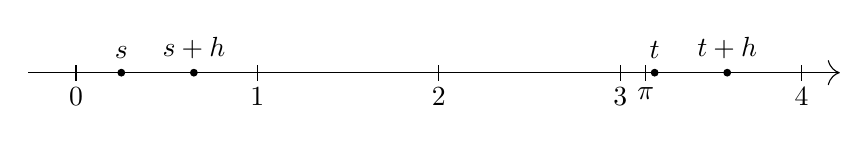
\begin{tikzpicture}[x=0.19\textwidth]
      \draw[-{>[scale=1.75]}] (-0.05\textwidth,0) -- (0.8\textwidth,0);
      \foreach \x in {0,...,4} {%
        \draw (\x,-.1) -- (\x,.1);
        \node[anchor=north,yshift=-2pt] at (\x,0) {$\x$};
      }
      \draw (3.141592654,-.1) -- (3.141592654,.1);
      \node[anchor=north,yshift=-2pt] at (3.141592654,0) {$\pi$};
      \draw (0.25,0) node [circle,fill,inner sep=1pt,label=above:$s$](e){};
      \draw (0.65,0) node [circle,fill,inner sep=1pt,label=above:$s+h$](e){};
      \draw (3.19,0) node [circle,fill,inner sep=1pt,label=above:$t$](e){};
      \draw (3.59,0) node [circle,fill,inner sep=1pt,label=above:$t+h$](e){};
    \end{tikzpicture}
  \end{image}
  Let $f(x) = \sin x$.  How does $f(s+h)-f(s)$ compare with $f(t+h) - f(t)$?
  \begin{multipleChoice}
    \choice{$f(s+h) - f(s) < f(t+h) - f(t)$}
    \choice{$f(s+h) - f(s) = f(t+h) - f(t)$}
    \choice[correct]{$f(s+h) - f(s) > f(t+h) - f(t)$}
  \end{multipleChoice}
\end{problem}



\section{Understanding functions}

\begin{problem}
\recommendation{Vic}
  Suppose $f(x) = x^2$.  How does $f(f(x))$ compare to $f(x)$?
  \begin{multipleChoice}
    \choice{Whenever $x$ is close to one, $f(f(x))$ is close to zero.}
    \choice{Whenever $x$ is close to one, $f(f(x))$ is larger than $x$.}
    \choice{Whenever $x$ is close to zero, $f(f(x))$ is larger than $x$.}
    \choice[correct]{Whenever $x$ is large, $f(f(x))$ is larger than $x$.}
  \end{multipleChoice}
\end{problem}

\begin{problem}
	Let $f$ and $g$ be two functions satisfying the relationship $f(x) = g(4x)$.  Suppose the point$(2,3)$ is on the graph of $f$.
	\begin{multipleChoice}
		\choice{The point $(\frac{1}{2},3)$ is on the graph of $g$}
		\choice[correct]{The point $(8, 3)$ is on the graph of $g$}
		\choice{The point $(8, 12)$ is on the graph of $g$}
		\choice{The point $(\frac{1}{2}, 12)$ is on the graph of $g$}
	\end{multipleChoice}
\end{problem}

\begin{problem}
	Let $f$ and $g$ be two functions satisfying the relationship $f(5x) = g(x)$.  Suppose the point $(1,2)$ is on the graph of $f$.
	\begin{multipleChoice}
		\choice{The point $(5, 2)$ is on the graph of $g$}
		\choice{The point $(5, 10)$ is on the graph of $g$}
		\choice{The point $(\frac{1}{5}, 10)$ is on the graph of $g$}
		\choice[correct]{The point $(\frac{1}{5},2)$ is on the graph of $g$}
	\end{multipleChoice}
\end{problem}

\begin{problem}
	Let $f$ and $g$ be two functions satisfying the relationship $f(x+3) = g(x)$.  Suppose the point $(0,0)$ is on the graph of $f$.
	\begin{multipleChoice}
		\choice[correct]{The point $(-3, 0)$ is on the graph of $g$}
		\choice{The point $(3, 0)$ is on the graph of $g$}
		\choice{The point $(0, 3)$ is on the graph of $g$}
		\choice[correct]{The point $(0,-3)$ is on the graph of $g$}
	\end{multipleChoice}
\end{problem}

\begin{problem}
	Could the points $(1,2)$,  $(4,5)$, $(5,5)$ all be points on the graph of the same function?
	\begin{multipleChoice}
		\choice[correct]{Yes}
		\choice{No}
	\end{multipleChoice}
\end{problem}

\begin{problem}
	Could the points $(4,2)$,  $(\pi,5)$, $(7,3)$, and $(4,3)$ all be points on the graph of the same function?
	\begin{multipleChoice}
		\choice{Yes}
		\choice[correct]{No}
	\end{multipleChoice}
\end{problem}

\begin{problem}
	Let $f$ be the function defined by $f(x) = x+1$, and $g$ be the function defined by the rule $g(u) = \frac{u^2-1}{u-1}$. 
	\begin{multipleChoice}
		\choice[correct]{Since $f$ and $g$ have differing domain, they are different functions}
		\choice{$f$ and $g$ are the same function}
		\choice{$f$ and $g$ are different functions because they disagree for some inputs in their common domain}
		\choice{$f$ and $g$ are different functions because they are of different variables}
	\end{multipleChoice}
\end{problem}

\begin{problem}
	Let $f$ be the function defined by $f(x) = x^2+1$, and $g$ be the function defined by the rule $g(z) = z^2+1$. 
	\begin{multipleChoice}
		\choice{Since $f$ and $g$ have differing domain, they are different functions}
		\choice[correct]{$f$ and $g$ are the same function}
		\choice{$f$ and $g$ are different functions because they disagree for some inputs in their common domain}
		\choice{$f$ and $g$ are different functions because they are of different variables}
	\end{multipleChoice}
\end{problem}

\begin{problem}
	Let $f$ be the function defined by $f(a) = \frac{a^2}{a}$, and $g$ be the function defined by the rule $g(z) = \frac{b^3}{b^2}$. 
	\begin{multipleChoice}
		\choice{Since $f$ and $g$ have differing domain, they are different functions}
		\choice[correct]{$f$ and $g$ are the same function}
		\choice{$f$ and $g$ are different functions because they disagree for some inputs in their common domain}
		\choice{$f$ and $g$ are different functions because they are of different variables}
	\end{multipleChoice}
\end{problem}

\begin{problem}
	Let $f$ be the function defined by $f(x) = \sqrt[4]{x^4}}$, and $g$ be the function defined by the rule $g(y) = \left| y \right|$. 
	\begin{multipleChoice}
		\choice{Since $f$ and $g$ have differing domain, they are different functions}
		\choice[correct]{$f$ and $g$ are the same function}
		\choice{$f$ and $g$ are different functions because they disagree for some inputs in their common domain}
		\choice{$f$ and $g$ are different functions because they are of different variables}
	\end{multipleChoice}
\end{problem}
\clearpage

\section{Review of famous functions}

\begin{problem}
\recommendation{Vic}
   Which of the following statements is true?
   \begin{multipleChoice}
     \choice{$\sin^{-1}(x)$ is the inverse function of $\sin(x)$} %this is perhaps a bit too subtle?
     \choice[correct]{$\sin\left(\sin^{-1}\left(\frac{1}{2}\right)\right) = \frac{1}{2}$} 
     \choice{$\sin^{-1}\left(\sin\left(\frac{5\pi}{2}\right)\right) = \frac{5\pi}{2}$}
     \choice{$\sin^{-1}(x) = \frac{1}{\sin(x)}$}
   \end{multipleChoice}  
\end{problem}

\begin{problem}
  The expression $\log_b(x) = y$ is equivalent to:
  \begin{multipleChoice}
    \choice{$b^x = y$}
    \choice[correct]{$b^y = x$}
    \choice{$x^b = y$}
    \choice{$x^y = b$}
    \choice{$y^b = x$}
    \choice{$y^x = b$}
  \end{multipleChoice}  
\end{problem}

\begin{problem}
  Suppose $f(x) = x \sin^2 x$.  What is true about $f$?
  \begin{multipleChoice}
    \choice[correct]{When $x$ is close to zero, $f(x)$ is close to zero.}
    \choice{When $x$ is very large, $f(x)$ is very large.}
    \choice{When $x$ is very negative, $f(x)$ is very negative.}
    \choice{When $x$ is close to one, $f(x)$ is close to one.}
  \end{multipleChoice}
\end{problem}

\begin{problem}
	Suppose $f(x) = \log(x+1) - \log(x)$.  What is true about $f$?
	\begin{multipleChoice}
       \choice{When $x$ is very large, $f(x)$ is very large.}
       \choice[correct]{When $x$ is very large, $f(x)$ is close to $0$.}
       \choice{When $x$ is close to $0$, $f(x)$ is close to $1$.}
       \choice{When $x$ is close to one, $f(x)$ is close to $0$.}
  \end{multipleChoice}
\end{problem}

\begin{problem}
	Is there an angle $\theta$ with $\sin(\theta) = \frac{1}{5}$ %Tests that they understand sine is not just the collection of 3 essentially different ``standard" values we have them memorize.
	\begin{multipleChoice}
		\choice[correct]{Yes}
		\choice{No}
	\end{multipleChoice}
\end{problem}

\begin{problem}
	Is there an angle $\theta$ with $\cos(\theta) = \frac{5}{4}$ ?
	\begin{multipleChoice}
		\choice{Yes}
		\choice[correct]{No}
	\end{multipleChoice}
\end{problem}

\begin{problem}
	Is there an angle $\phi$ with $\sin(\phi) = \frac{5}{13}$ and $\cos(\phi) = -\frac{12}{13}$?
	\begin{multipleChoice}
		\choice[correct]{Yes}
		\choice{No}
	\end{multipleChoice}
\end{problem}

\begin{problem}
	Is there an angle $y$ with $\sin(y) = \frac{4}{5}$ and $\cos(y) = \frac{1}{5}$?
	\begin{multipleChoice}
		\choice{Yes}
		\choice[correct]{No}
	\end{multipleChoice}
\end{problem}

\clearpage

\section{What is a limit?}

\begin{problem}
\recommendation{Vic}
  Suppose $x$ is a positive number close to zero, and $y$ is a very large number.  What can be said about $y/x$?
  \begin{multipleChoice}
    \choice[correct]{It is very large.}
    \choice{It is close to zero.}
    \choice{It is very negative.}
    \choice{It could be very positive or very negative.}
  \end{multipleChoice}
\end{problem}

\begin{problem}
  Suppose $x$ is a number close to zero.  What can be said about $1/x^3$?
  \begin{multipleChoice}
    \choice{It is very large.}
    \choice{It is close to zero.}
    \choice{It is very negative.}
    \choice[correct]{It could be very positive or very negative.}
  \end{multipleChoice}
\end{problem}

\begin{problem}
  Suppose $x$ is a number close to zero.  What can be said about $1/x^4$?
  \begin{multipleChoice}
    \choice[correct]{It is very large.}
    \choice{It is close to zero.}
    \choice{It is very negative.}
    \choice{It could be very positive or very negative.}
  \end{multipleChoice}
\end{problem}

\begin{problem}
	Suppose $x$ is a small negative number.  What can be said about $\frac{x}{|x|}$?
	\begin{multipleChoice}
		\choice[correct]{It is close to $-1$}
		\choice{It is close to $1$}
		\choice{It is close to $0$}
	\end{multipleChoice}
\end{problem}

\begin{problem}
  Suppose $x$ is a number close to zero, and $y$ is a very large number.  What can be said about $y/x$?
  \begin{multipleChoice}
    \choice{It is very large.}
    \choice{It is close to zero.}
    \choice{It is very negative.}
    \choice[correct]{It could be very positive or very negative.}
  \end{multipleChoice}
\end{problem}

\begin{problem}
  Suppose $x$ and $y$ are numbers close to zero.  What can be said about $x+y$?
  \begin{multipleChoice}
    \choice[correct]{It is close to zero.}
    \choice{It is negative.}
    \choice{It is positive.}
    \choice{It is larger than $x$ and larger than $y$.}
  \end{multipleChoice}
\end{problem}

\begin{problem}
  Suppose $x = 10^{100}$ and $y = 10^{1000}$.  Which number below is closest to $x + y$?
  \begin{multipleChoice}
    \choice{$1000 + 10^{100}$}
    \choice{$10^{100}$}
    \choice[correct]{$10^{1000}$}
    \choice{$10^{1100}$}
  \end{multipleChoice}
\end{problem}

\begin{problem}
	I start with $0.3$.  I add $0.03$ to it.  Then I add $0.003$.  Then $0.0003$.  I keep adding numbers for a very long time.  What happens to the sum as I add more terms?
	\begin{multipleChoice}
		\choice{The sum gets very large.  If I went long enough, the sum would surpass $10$}
		\choice{The sum never gets very large.  It would never surpass $1$, no matter how many terms I summed}
		\choice{The sum of the terms gets closer to $0$}
	\end{multipleChoice}
\end{problem}

\clearpage

\section{Limit laws}

\begin{problem}
  Suppose $x$ is close to $0$ and $y$ is close to $-2$.  What is necessarily true about $xy$?
  \begin{multipleChoice}
    \choice[correct]{It is close to zero and could be either negative or positive}
    \choice{It is close to zero and must be positive}
    \choice{It is close to zero and must be negative}
    \choice{It is smaller than $y$.}
  \end{multipleChoice}
\end{problem}

\begin{problem}
  % BADBAD draw this on a number line
  Suppose $x$ is close to $0$ and $y$ is close to $-2$ and $z$ is close to $2$.  What is true about these numbers?
  \begin{multipleChoice}
    \choice{$y/x < z/x$}
    \choice[correct]{$y/x^4 < z/x^2$}
    \choice{$y/x^5 < z/x^3$}
    \choice{$y/x^5 < z/x^5$}
  \end{multipleChoice}
\end{problem}

\begin{problem}
	%This problem would be a real stretch for someone who has not seen limits, or the derivative, already.
  Suppose $x$ is $0.000001$ and $y = 10$ and $z = 9$.  Which is larger:
  $A = \frac{\sin (yx)}{zx}$ or $B = \frac{\sin (zx)}{yx}$?
  \begin{multipleChoice}
    \choice[correct]{$A$ is larger than $B$.}
    \choice{$B$ is larger than $A$.}
  \end{multipleChoice}
\end{problem}

\begin{problem}
	%This problem would be a real stretch for someone who has not seen limits, or the derivative, already.
  Suppose $x$ is $0.00\dots 0017$ with $10^{17}$ zeroes after the
  decimal point, and suppose $y$ and $z$ are large positive integers
  with $y > z$.  Which is larger: $A = \frac{\sin (yx)}{zx}$ or
  $B = \frac{\sin (zx)}{yx}$?
  \begin{multipleChoice}
    \choice[correct]{$A$ is larger than $B$.}
    \choice{$B$ is larger than $A$.}
  \end{multipleChoice}
\end{problem}

\begin{problem}
  Pick some positive real number; take its square root, and then the
  square root of that, and then the square root of that, and so
  on---thousands and thousands of times.  Call the result $x$.  What
  do you expect to be true of $x$?
  \begin{multipleChoice}
    \choice{The number $x$ is close to $0$.}
    \choice[correct]{The number $x$ is close to $1$.}
    \choice{The number $x$ is very large.}
  \end{multipleChoice}
\end{problem}

\begin{problem}
  Pick some positive real number; add one; take its square root, and
  then add one and take the square root of that, and then add one and
  again take the square root of that, and so on---thousands and
  thousands of times.  Call the result $x$.  What do you expect to be
  true of $x$?
  \begin{multipleChoice}
    \choice{The number $x$ is close to $0$.}
    \choice{The number $x$ is close to $1$.}
    \choice[correct]{The number $x$ is between $1$ and $2$.}
    \choice{The number $x$ is very large.}
  \end{multipleChoice}
\end{problem}



\clearpage

\section{Indeterminate forms}

\begin{problem}
  When $x = 10^{100}$, what number below is closest to $\sqrt{x^2 + x}$?
  \begin{multipleChoice}
    \choice{$10^{50}$}
    \choice[correct]{$10^{100}$}
    \choice{$10^{100} + 10^{200}$}
    \choice{$10^{200}$}
  \end{multipleChoice}
\end{problem}

\begin{problem}
  When $x = 10^{1000}$, what number below is closest to $\frac{2x^2 - 1}{x-2}$? % = 2x + 4 + small
  \begin{multipleChoice}
    \choice{$x$}
    \choice{$x - 4$}
    \choice{$x + 4$}
    \choice{$2$}
    \choice[correct]{$2x$}
  \end{multipleChoice}
\end{problem}

\begin{problem}
  %This seems difficult without advanced knowledge of sine.
  When $x = \pi^{-1000}$, what number below is closest to $\frac{\sin \sin x}{x}$?
  \begin{multipleChoice}
    \choice{$-1$}
    \choice{$0$}
    \choice[correct]{$1$}
    \choice{This quantity is undefined}
  \end{multipleChoice}
\end{problem}

\begin{problem}
  Suppose $A$ and $a$ differ by at most $2$ and suppose $B$ and $b$
  differ by at most $1$.  In symbols, this means that $|A - a| < 2$ and $|B - b| < 1$.
  By how much could $A/B$ and $a/b$ differ?
  \begin{multipleChoice}
    \choice{By no more than $1$, meaning $|A/B - a/b| < 1$}
    \choice{By no more than $2$, meaning $|A/B - a/b| < 2$}
    \choice{By no more than a factor of $2$, meaning $\left| \frac{A/B}{a/b} \right| < 2$}
    \choice{By no more than a factor of $1/2$, meaning $\left| \frac{A/B}{a/b} \right| < \frac{1}{2}$}
    \choice[correct]{By any amount}
  \end{multipleChoice}
\end{problem}

\begin{problem}
  By choosing $x$ appropriately, how large can $1/x^2$ be?
  \begin{multipleChoice}
    \choice{The quantity $1/x^2$ can be no bigger than $1$.}
    \choice[correct]{The quantity $1/x^2$ can be made as large as desired.}
  \end{multipleChoice}
\end{problem}

\begin{problem}
\recommendation{Vic}
	%Difficult without advanced sine knowledge
  Suppose $x = 3 \cdot 10^{-1000}$ and $y = 6 \cdot 10^{-1000}$.  What is the best guess for $\frac{\sin (xy)}{x^2}$?
  \begin{multipleChoice}
    \choice{$0$}
    \choice{$1$}
    \choice[correct]{$2$}
    \choice{$3$}
  \end{multipleChoice}
\end{problem}

\begin{problem}
	%Difficult without advanced sine knowledge

  Suppose $x = 5 \cdot 10^{-1000}$ and $y = 2 \cdot 10^{-999}$.  What is the best guess for $\frac{\sin (xy)}{x^2}$?
  \begin{multipleChoice}
    \choice{$0$}
    \choice{$1$}
    \choice{$2$}
    \choice{$3$}
    \choice[correct]{$4$}
  \end{multipleChoice}
\end{problem}

\begin{problem}
  By choosing $x$ appropriately, how small can $f(x) = \frac{1}{\sin (x^2)}$ be?
  \begin{multipleChoice}
    \choice{The quantity $f(x)$ cannot be negative}
    \choice{The quantity $f(x)$ must be larger than $-1$ but can take negative values}
    \choice[correct]{The quantity $f(x)$ can be made as negative as desired}
  \end{multipleChoice}
\end{problem}

\clearpage

\section{Using limits to detect asymptotes}

\begin{problem}
  Suppose whenever $x$ is very large, $f(x)$ is close to 1.  What is true about $f$?
  \begin{multipleChoice}
    \choice{The graph of $f$ does not cross the line $y = 1$.}
    \choice{The graph of $f$ does not cross the line $x = 1$.}
    \choice{Whenever $x$ is close to zero, $f(1/x)$ is close to 1.}
    \choice[correct]{Whenever $x$ is very large, $f(x^2)$ is close to 1.}
  \end{multipleChoice}
\end{problem}

\begin{problem}
  For a certain function $f$ with domain consisting of all real
  numbers, it is the case that $f(x) < 0$ and yet $f$ is increasing.
  What must be true of $f$?
  \begin{multipleChoice}
    \choice{The graph of $f$ has a horizontal asymptote at $y = 0$}
    \choice{$\lim_{x \to -\infty} f(x) = -\infty$}
    \choice{$\lim_{x \to \infty} f(x)$ exists and is negative}
    \choice[correct]{None of these statements need be true}
  \end{multipleChoice}
\end{problem}

\begin{problem}
  Consider the function $f(x) = \log_{10} \log_{10} \log_{10} x$.  On my calculator, I notice that $f(10^{100}) \approx 0.3$.  What is true about $f$?
  \begin{multipleChoice}
    \choice{$\lim_{x \to \infty} f(x) = -\infty$}
    \choice{$\lim_{x \to \infty} f(x)$ exists and is a negative real number}
    \choice{$\lim_{x \to \infty} f(x) = 0$}
    \choice{$\lim_{x \to \infty} f(x) = 0.5$}
    \choice{$\lim_{x \to \infty} f(x) = 1$}
    \choice[correct]{$\lim_{x \to \infty} f(x) = \infty$}
  \end{multipleChoice}  
\end{problem}

\begin{problem}
  Suppose $f$ is a function and $f(x) > 0$ and $\lim_{x \to \infty} f(x) = 0$ and $\lim_{x \to 0} f(x) = 1$.  When $x$ is a small positive number, what do you expect to be true about $1/f(1/x)$?
  \begin{multipleChoice}
    \choice{It is very negative}
    \choice{It is close to $-1$}
    \choice{It is close to $0$}
    \choice{It is close to $1$}
    \choice[correct]{It is very large}
  \end{multipleChoice}
\end{problem}

\clearpage

\section{Continuity and the Intermediate Value Theorem}

\begin{problem}
  Suppose $f$ and $g$ are continuous functions.  Let $h(x) = \frac{f(x+0.01) \cdot g(x - 0.01)}{f(x-0.02) \cdot f(x + 0.02)}$.  Without knowing anything else, what number below is the best guess for $h(2)$?
  \begin{multipleChoice}
    \choice{$f(2)$}
    \choice{$g(2)$}
    \choice{$f(2)/g(2)$}
    \choice[correct]{$g(2)/f(2)$}
  \end{multipleChoice}
\end{problem}

\begin{problem}
  Define $f(x) = x \cos x + sin\left(\frac{x^{10}}{10^{100}}\right)$.  What number below is closest to $f(3)$?
  \begin{multipleChoice}
    \choice[correct]{$-3$}
    \choice{$-1$}
    \choice{$0$}
    \choice{$1$}
    \choice{$3$}
  \end{multipleChoice}
\end{problem}

\begin{problem}
\recommendation{Vic}
  Suppose $f$ is a function and that $\lim_{h \to 0^{+}} f(h) = \lim_{h \to 0^{-}} f(h)$.  What is true about $f$?
  \begin{multipleChoice}
    \choice[correct]{The function $f$ need not be continuous at $0$.}
    \choice{The function $f$ is continuous at $0$ because the left and right hand limits agree.}
  \end{multipleChoice}
\end{problem}

\begin{problem}
\recommendation{Vic}
  Suppose $f$ is a function which is not differentiable at a point $a$.  Then what is true about $f$?
  \begin{multipleChoice}
    \choice{The function $f$ is not continuous at $a$}
    \choice[correct]{The function $f$ could be continuous at $a$}
  \end{multipleChoice}
\end{problem}

\begin{problem}
  Suppose $f$ is a function so that whenever $0 \leq x \leq 1$ then
  $0 \leq f(x) \leq 1$.  Moreover, for all $y$ between $0$ and $1$
  there is some $x$ so that $f(x) = y$.  Must $f$ then be continuous?
  \begin{multipleChoice}
    \choice[correct]{No}
    \choice{Yes}
  \end{multipleChoice}
\end{problem}

\begin{problem}
  For $0 \leq x \leq \pi$, define
  $f(x) = \lim_{n \to \infty} \sin^n x$.  What is true about $f$?
  \begin{multipleChoice}
    \choice{The function $f$ is continuous}
    \choice[correct]{The function $f$ is not continuous}
  \end{multipleChoice}
\end{problem}

\begin{problem}
  For $0 \leq x \leq 1$, define
  $f(x) = \lim_{n \to \infty} x^n$.  What is true about $f$?
  \begin{multipleChoice}
    \choice{The function $f$ is continuous}
    \choice[correct]{The function $f$ is not continuous}
  \end{multipleChoice}
\end{problem}

\begin{problem}
  Say a function ``misses zero'' if there is no number $x$ so that
  $f(x) = 0$.  Among functions which miss zero, how large can $1/f(x)$
  be?
  \begin{multipleChoice}
    \choice{If a given function $f$ misses zero, then $1/f(x)$ can be made as large as desired.}
    \choice[correct]{There are functions which miss zero, and yet for all $x$, it is the case that $1/f(x) < 1$.}
    \choice{The quantity $1/f(x)$ is undefined for functions $f$ which miss zero.}
  \end{multipleChoice}
\end{problem}

\begin{problem}
  Suppose $f$ is a continuous function so that whenever $0 \leq x \leq 1$ we have $0 \leq f(x) \leq 1$.  What must be true about $f$?
  \begin{multipleChoice}
    \choice[correct]{There is an $x$ so that $f(x) = x$.}
    \choice{There is an $x$ so that $f(x) > 1$.}
    \choice{There is an $x$ so that $f(x) > x$.}
    \choice{There is an $x$ so that $f(x) < 0$.}
    \choice{There is an $x$ so that $f(x) < x$.}
  \end{multipleChoice}
\end{problem}

\clearpage

\section{An Application of limits}

\begin{problem}
  What integer is closest to $\frac{\ln 0.26 - \ln 0.25}{0.01}$?
  \begin{multipleChoice}
    \choice{$100$}
    \choice{$25$}
    \choice{$5$}
    \choice[correct]{$4$}
    \choice{$0$}
  \end{multipleChoice}
\end{problem}

\begin{problem}
  What integer is closest to $\frac{\ln 1.26 - \ln 1.25}{0.004}$?
  \begin{multipleChoice}
    \choice{$3$}
    \choice[correct]{$2$}
    \choice{$1$}
    \choice{$0$}
  \end{multipleChoice}
\end{problem}

\begin{problem}
  Suppose $f$ is a differentiable function and $f(0) = 0$.  When $h$
  is a number close to zero, what do you expect $\frac{f(h)}{h}$ is
  closest to?
  \begin{multipleChoice}
    \choice{$f(0)$}
    \choice{$h$}
    \choice{$f(h)$}
    \choice[correct]{$f'(0)$}
    \choice{$f''(0)$}
  \end{multipleChoice}
\end{problem}

\begin{problem}
  Suppose $f$ is a differentiable function.  When $h$ is a number
  close to zero, what do you expect $\frac{f(4h)}{2h}$ is close to?
  \begin{multipleChoice}
    \choice{$\frac{1}{4} \, f'(0)$}
    \choice{$\frac{1}{2} \, f'(0)$}
    \choice{$f'(0)$}
    \choice[correct]{$2 \, f'(0)$}
    \choice{$4 \, f'(0)$}
  \end{multipleChoice}
\end{problem}

\clearpage

\section{Definition of the derivative}

\begin{problem}
  Let $x = e^{10001} - e^{10000}$ and $y = e^{10002} - e^{10001}$.  How do $x$ and $y$ compare?
  \begin{multipleChoice}
    \choice[correct]{$x < y$}
    \choice{$x = y$}
    \choice{$x > y$}
  \end{multipleChoice}
\end{problem}

\begin{problem}
\recommendation{Vic}
  Let $f(x) = x^{800}$.  How does $A = f(10^{10} + 1)$ compare to $B = f(10^{10} - 1)$?
  \begin{multipleChoice}
    \choice{$A < B$}
    \choice{$A = B$}
    \choice[correct]{$A > B$}
  \end{multipleChoice}
\end{problem}

\begin{problem}
  Let $f(x) = x^{800}$.  How does $A = f(10^{10} + 1) - f(10^{10})$ compare to $B = f(10^{10}) - f(10^{10} - 1)$?
  \begin{multipleChoice}
    \choice{$A < B$}
    \choice{$A = B$}
    \choice[correct]{$A > B$}
  \end{multipleChoice}
\end{problem}

\begin{problem}
  Let $x = \log_b 1001 - \log_b 1000$ and $y = \log_b 101 - \log_b 100$.  How do $x$ and $y$ compare?
  \begin{multipleChoice}
    \choice[correct]{$x < y$}
    \choice{$x = y$}
    \choice{$x > y$}
    \choice{It depends on the base $b$.}
  \end{multipleChoice}
\end{problem}

\begin{problem}
\recommendation{Vic}
  Suppose $f$ and $g$ are differentiable functions and $f(1) = g(1)$ and 
  $0 > f'(1) > g'(1)$.  Based only on this information, which quantity
  do you expect to be largest?
  \begin{multipleChoice}
    \choice{$f'(1.02)$}
    \choice{$g'(1.02)$}
    \choice{$f'(0.99)$}
    \choice[correct]{$g'(0.99)$}
  \end{multipleChoice}
\end{problem}

\clearpage

\section{The derivative as a function}

\begin{problem}
  From far away, the graph of $f$ looks like the straight line
  $y = x$.  Close up, it looks very wiggly.  To be precise, $f(x) - x$
  is very close to zero.  What can be said about $f'(x)$?
  \begin{multipleChoice}
    \choice{The derivative $f'(x)$ is close to $\sin x$.}
    \choice{The derivative $f'(x)$ is close to $0$.}
    \choice{The derivative $f'(x)$ is close to $1$.}
    \choice[correct]{None of these statements are true}
  \end{multipleChoice}
\end{problem}

\clearpage

\section{Higher order derivatives and graphs}

\begin{problem}
\recommendation{Vic}
  Suppose $f$ and $g$ have the same second derivative at every point.  
  \begin{multipleChoice}
    \choice[correct]{It is possible that $f$ is increasing at $1$ and $g$ is decreasing at $1$.}
    \choice{Either $f$ and $g$ are both increasing or both decreasing at $1$.}
  \end{multipleChoice}
\end{problem}

\clearpage

\section{Rules of differentiation}

\begin{problem}
  Suppose $p(x) = x^2 + bx + c$ is a quadratic polynomial.  If $c > 0$, is it possible that there is a point $x$ so that $p'(x) = p(x) = 0$?
  \begin{multipleChoice}
    \choice[correct]{Yes}
    \choice{No}
  \end{multipleChoice}
\end{problem}

\begin{problem}
\recommendation{Vic}
  Suppose $p(x) = x^2 + a$ is a quadratic polynomial.  If $a > 0$, is it possible that there is a point $x$ so that $p'(x) = p(x) = 0$?
  \begin{multipleChoice}
    \choice{Yes}
    \choice[correct]{No}
  \end{multipleChoice}
\end{problem}

\clearpage

\section{The product and quotient rules}

\begin{problem}
  Suppose $A$ is just a big bigger than $a$ and $B$ is just a bit
  bigger than $b$.  To be more precise, $A > a$ and $B > b$ but
  $A - a$ and $B-b$ are close to zero.  How does $AB$ compare to $ab$?
  \begin{multipleChoice}
    \choice{$AB$ is bigger than $ab$}
    \choice{$AB$ is equal to $ab$}
    \choice{$AB$ is smaller than $ab$}
    \choice[correct]{It could be that $AB$ or $ab$ is larger}
  \end{multipleChoice}
\end{problem}

\begin{problem}
  Suppose $a$ and $b$ and $A$ and $B$ are very large, positive numbers, and suppose $A > a$ and $B > b$.  How does $A/B$ compare to $a/b$?
  \begin{multipleChoice}
    \choice{$A/B$ is bigger than $a/b$}
    \choice{$A/B$ is equal to $a/b$}
    \choice{$A/B$ is smaller than $a/b$}
    \choice[correct]{It could be that $A/B$ or $a/b$ is larger}
  \end{multipleChoice}
\end{problem}

\begin{problem}
  Suppose $a$ and $b$ and $A$ and $B$ are very large, positive numbers, and suppose $A > a$ and $B < b$.  How does $A/B$ compare to $a/b$?
  \begin{multipleChoice}
    \choice[correct]{$A/B$ is bigger than $a/b$}
    \choice{$A/B$ is equal to $a/b$}
    \choice{$A/B$ is smaller than $a/b$}
    \choice{It could be that $A/B$ or $a/b$ is larger}
  \end{multipleChoice}
\end{problem}

\clearpage

\section{The chain rule}

\begin{problem}
\recommendation{Vic}
  Suppose $f(x) = e^x$ so that $f'(x) = f(x)$.  Let $g(x) = e^{f(x)}$.  What is $g'(x)$?
  \begin{multipleChoice}
    \choice{$g'(x) = e^{(x e^x)}$ by the chain rule}
    \choice[correct]{$g'(x) = e^{(x + e^x)}$ by the chain rule}
    \choice{$g'(x) = e^{(e^x)}$ by the chain rule}
  \end{multipleChoice}
\end{problem}

\begin{problem}
  Suppose $f$ and $g$ are differentiable functions and $f(0) = 0$ and
  $g(0) = 0$ and when $h$ is close to zero, $f(g(h))$ is close to $6h$
  and $g(g(h))$ is close to $9h$.  What is a good approximation for $f(f(h))$?
  \begin{multipleChoice}
    \choice{$f(f(h))$ is close to $2h$}
    \choice{$f(f(h))$ is close to $3h$}
    \choice[correct]{$f(f(h))$ is close to $4h$}
  \end{multipleChoice}
\end{problem}

\begin{problem}
  Suppose $f$ is a differentiable function and $f(0) = 0$ and
  $f(\sin 0.03) = 6$.  What is a best guess for $f(0.01)$?
  \begin{multipleChoice}
    \choice[correct]{$2$}
    \choice{$4$}
    \choice{$6$}
  \end{multipleChoice}
\end{problem}

\begin{problem}
  Suppose $f$ is a differentiable function and $f(0) = 0$ and
  $f(\sin \frac{\pi}{100}) = 9$.  What number below is the best guess for $f(0.01)$?
  \begin{multipleChoice}
    \choice{$1$}
    \choice[correct]{$3$}
    \choice{$4$}
    \choice{$6$}
    \choice{$9$}
  \end{multipleChoice}
\end{problem}

\clearpage

\section{Mean Value Theorem}

\begin{problem}
\recommendation{Vic}
  Suppose $f$ is a differentiable function with domain the real numbers; further suppose that $f(0) = 0$ and that $f'(x) < 1$ for all $x$.  What is a possible value for $f(0.9999)$?
  \begin{multipleChoice}
    \choice[correct]{$0.99$}
    \choice{$0.99999$}
    \choice{$1.00$}
    \choice{$1.0001$}
  \end{multipleChoice}
\end{problem}

\begin{problem}
  On a car trip that took about 65 minutes, you spent some time
  driving about 65~mph and some time driving about 15~mph, but your
  average speed was about 40~mph.  How long did you spend driving
  around 15~mph?
  \begin{multipleChoice}
    \choice{About $15$ minutes}
    \choice[correct]{About $32$ minutes}
    \choice{About $40$ minutes}
    \choice{It depends on the distance traveled}
  \end{multipleChoice}
\end{problem}

\begin{problem}
  On a recent car trip, you spent some time driving about 65~mph and
  some time driving about 15~mph, but your average speed was about
  40~mph.  How long did you spend driving at 15~mph versus 65~mph?
  \begin{multipleChoice}
    \choice{Nearly the entire time was spent driving 15~mph}
    \choice{About half the time}
    \choice{Nearly the entire time was spent driving 65~mph}
    \choice{It depends on the distance traveled}
  \end{multipleChoice}
\end{problem}

\begin{problem}
\recommendation{Vic}
  Suppose $f$ is an increasing function, and $x$ and $h$ are positive numbers between $0$ and $1$.  How does $f(x + h)$ compare to $f(x + h^2)$?
  \begin{multipleChoice}
    \choice[correct]{$f(x+h) > f(f+h^2)$}
    \choice{$f(x+h) < f(f+h^2)$}
    \choice{It depends on the function $f$.}
  \end{multipleChoice}
\end{problem}

\begin{problem}
  Suppose $f$ and $g$ are increasing functions.  What can be said about the function $h(x) = f(g(x))$?
  \begin{multipleChoice}
    \choice[correct]{It is an increasing function.}
    \choice{It is a decreasing function.}
    \choice{It depends on exactly which functions $f$ and $g$ are being considered.}
  \end{multipleChoice}
\end{problem}

\begin{problem}
  Suppose $f$ and $g$ are decreasing functions.  What can be said about the function $h(x) = f(g(x))$?
  \begin{multipleChoice}
    \choice[correct]{It is an increasing function.}
    \choice{It is a decreasing function.}
    \choice{It depends on exactly which functions $f$ and $g$ are being considered.}
  \end{multipleChoice}
\end{problem}

\begin{problem}
  For a certain function $f$, both $f(x) > 0$ and $f'(x) > 0$ for all $x$.  Let $g(x) = \frac{1}{-f(-x)}$.  What can be said about $g'(x)$?
  \begin{multipleChoice}
    \choice[correct]{For all $x$ it is the case that $g'(x) < 0$}
    \choice{For all $x$ it is the case that $g'(x) = 0$}
    \choice{For all $x$ it is the case that $g'(x) > 0$}
    \choice{It depends---depending on $f$ and on $x$, it could be that $g'(x) > 0$ or $g'(x) < 0$}
  \end{multipleChoice}
\end{problem}

\clearpage

\section{Linear approximation}

\begin{problem}
\recommendation{Vic}
  Suppose $y = mx + b$ is the equation for a tangent line at the point $(100,\log 100)$ to the graph of $f(x) = \log x$.  How does $200m + b$ compare to $\log 200$?
  \begin{multipleChoice}
    \choice[correct]{$200m + b > \log 200$}
    \choice{$200m + b < \log 200$}
    \choice{$200m + b = \log 200$}
  \end{multipleChoice}
\end{problem}

\begin{problem}
  Suppose $y = mx + b$ is the equation for a tangent line at the point $(100,e^{100})$ to the graph of $f(x) = e^x$.  How does $200m + b$ compare to $e^{200}$?
  \begin{multipleChoice}
    \choice{$200m + b > e^{200}$}
    \choice[correct]{$200m + b < e^{200}$}
    \choice{$200m + b = e^{200}$}
  \end{multipleChoice}
\end{problem}

\clearpage

\section{Maximums and minimums}

\begin{problem}
\recommendation{Vic}
  Suppose $f$ is a continuous function on the interval $(-1,1)$ and suppose $f(0) = 0$.  How large could $f(0.9999)$ be?
  \begin{multipleChoice}
    \choice[correct]{Bigger than $1$}
    \choice{No bigger than $1$ but it could be very negative}
    \choice{Anywhere between $-1$ and $1$ but not outside this range}
  \end{multipleChoice}
\end{problem}

\begin{problem}
  Suppose a smooth function $f$ with domain the real numbers has the property that $-1 \leq f(x) \leq 1$ for all $x$.  What is true of $f$?
  \begin{multipleChoice}
    \choice[correct]{$f$ need not achieve a global maximum value}
    \choice{$f$ achieves a global maximum value}
  \end{multipleChoice}
\end{problem}

\begin{problem}
  Suppose a continuous function $f$ with domain the real numbers has infinitely many local minima.  What is true of $f$?
  \begin{multipleChoice}
    \choice[correct]{$f$ has infinitely many local maxima.}
    \choice{$f(x)$ can be made as large as desired by choosing appropriate $x$}
    \choice{$f(x)$ can be made as small as desired by choosing appropriate $x$}
    \choice{None of these statements are true.}
  \end{multipleChoice}
\end{problem}

\begin{problem}
  Let $f(x) = x^2 \sec^2 x$.  What is true of $f$?
  \begin{multipleChoice}
    \choice{$f$ has exactly one local minimum.}
    \choice{$f$ has exactly one local maximum.}
    \choice[correct]{$f$ has infinitely many local minima.}
    \choice{$f$ has infinitely many local maxima.}
  \end{multipleChoice}
\end{problem}

\begin{problem}
  Suppose a function $f$ has no global maximum value.  What is true of $f$?
  \begin{multipleChoice}
    \choice{$f$ has infinitely many local minima.}
    \choice{$f(x)$ can be made as large as desired by choosing appropriate $x$}
    \choice{$f(x)$ can be made as small as desired by choosing appropriate $x$}
    \choice[correct]{None of these statements are true.}
  \end{multipleChoice}
\end{problem}

\begin{problem}
  Suppose a polynomial $f$ achieves a global minimum, and besides that
  one point has no other local or global extrema.  What must be true
  of $f$?
  \begin{multipleChoice}
    \choice{$f'$ is a constant function}
    \choice{$f''$ is a constant function but it could be either negative or positive}
    \choice{$f''$ is a constant function and must be positive}
    \choice[correct]{None of these statements are true.}
  \end{multipleChoice}
\end{problem}

\clearpage

\section{Optimization}

\begin{problem}
\recommendation{Vic}
  Suppose $f$ has a local minimum at $(m,f(m))$.  Let $g(x) = f(x) \cdot f(x)$.  What can be said about $g$?
  \begin{multipleChoice}
    \choice{The function $g$ must have a local minimum at $(m,g(m))$}
    \choice{The function $g$ must have a local maximum at $(m,g(m))$}
    \choice[correct]{The function $g$ must have either a local maximum or a local minimum at $(m,g(m))$}
    \choice{None of these statements are true.}
  \end{multipleChoice}
\end{problem}

\begin{problem}
  Suppose $f(m)$ is the minimum value of a function $f$.  Let $g(x) = -f(x) \cdot f(x)$.  What must be true about $g$?
  \begin{multipleChoice}
    \choice{$f(m)^2$ is the minimum value of $g$}
    \choice{$f(m)^2$ is the maximum value of $g$}
    \choice[correct]{$f(m)^2$ need not be the maximum or minimum value of $g$}
  \end{multipleChoice}
\end{problem}

\begin{problem}
  Suppose $f$ has a local minimum at $(0,f(0))$ and at $f(1,f(1))$.  What must be true about $f$?
  \begin{multipleChoice}
    \choice{There is some value of $x$ so that $(x,f(x))$ is a local maximum}
    \choice{There is some value of $x$ so that $(x,f(x))$ is a global minimum}
    \choice{There is some value of $x$ so that $(x,f(x))$ is a global maximum}
    \choice[correct]{None of these statements are necessarily true.}
  \end{multipleChoice}
\end{problem}

\begin{problem}
  Suppose $f$ is a continuous function which has a local minimum at $(0,f(0))$ and at $f(1,f(1))$.  What must be true about $f$?
  \begin{multipleChoice}
    \choice[correct]{There is some value of $x$ so that $(x,f(x))$ is a local maximum}
    \choice{There is some value of $x$ so that $(x,f(x))$ is a global minimum}
    \choice{There is some value of $x$ so that $(x,f(x))$ is a global maximum}
    \choice{None of these statements are necessarily true.}
  \end{multipleChoice}
\end{problem}

\clearpage

\section{Applied optimization}

\clearpage

\section{Derivatives of trigonometric functions}

\begin{problem}
  Suppose a function $f$ has the property that $f'' = -f$.  What is true of $f$?
  \begin{multipleChoice}
    \choice{$f(x) = \cos x$}
    \choice[correct]{$f^{(4)}(x) = f(x)$}
    \choice{$f(x) = \tan x$}
    \choice{$f^{(4)}(x) = -f(x)$}
  \end{multipleChoice}
\end{problem}

\begin{problem}
  How does $\sin(0.01)$ compare to $\sin(3.14)$?
  \begin{multipleChoice}
    \choice{$\sin(0.01) > 0 > \sin(3.14)$}
    \choice[correct]{$\sin(0.01) > \sin(3.14) > 0$}
    \choice{$\sin(3.14) > \sin(0.01) > 0$}
    \choice{$\sin(3.14) > 0 > \sin(0.01)$}
  \end{multipleChoice}
\end{problem}

\begin{problem}
  Pick a large number $x$ and a number $h$ very close to $0$ so that $0 > \sin x > \sin (x+h)$.  How might $\cos (x+h)$ compare to $\cos x$?
  \begin{multipleChoice}
    \choice[correct]{$\cos (x+h) > \cos x$}
    \choice{$\cos (x+h) = \cos x$}
    \choice{$\cos (x+h) < \cos x$}
  \end{multipleChoice}
\end{problem}

\clearpage

\section{Implicit differentiation}

\begin{problem}
  Suppose $f$ is an increasing function and $f(x) \cdot g(x)$ is a constant.  How does $g$ depend on $x$?
  \begin{multipleChoice}
    \choice{$g$ must be increasing}
    \choice[correct]{$g$ could be constant}
    \choice{$g$ must be decreasing}
  \end{multipleChoice}
\end{problem}

\begin{problem}
\recommendation{Vic}
  Suppose $f(x)^2 + g(x)^2 = 10$ and suppose $f'(a) > 0$.  What must be true about $g'(a)$?
  \begin{multipleChoice}
    \choice{$g'(a) > 0$}
    \choice{$g'(a) = 0$}
    \choice{$g'(a) < 0$}
    \choice[correct]{None of the above statements are necessarily true.}
  \end{multipleChoice}
\end{problem}

\clearpage

\section{Derivatives of inverse functions}

\begin{problem}
\recommendation{Vic}
  There is a function $f$ so that $f(0) = 0$ and when $h$ is small, $f^{-1}(h)$ is close to $10 h$.  What is a good guess for $f'(0)$?
  \begin{multipleChoice}
    \choice{$10$}
    \choice{$-10$}
    \choice[correct]{$1/10$}
    \choice{$-1/10$}
  \end{multipleChoice}
\end{problem}

\begin{problem}
\recommendation{Vic}
  Suppose $f$ is a function and $f'(0) = 0$.  What is true about $f$?
  \begin{multipleChoice}
    \choice{$f$ can not be an invertible function}
    \choice[correct]{$f$ could be an invertible function}
  \end{multipleChoice}
\end{problem}

\clearpage

\section{Logarithmic differentiation}

\begin{problem}
  Consider a positive continuous function $f$ and its logarithmic derivative $g(x) = \frac{f'(x)}{f(x)}$.  Suppose $g(x) = 0.05$ when $0 < x < 10$ and $g(x) = -0.05$ when $10 < x < 20$.  How do $f(0)$ and $f(20)$ compare?
  \begin{multipleChoice}
    \choice[correct]{$f(20) > f(0)$}
    \choice{$f(0) < f(20)$}
    \choice{$f(0) = f(20)$}
  \end{multipleChoice}
\end{problem}

\clearpage

\section{Advanced graphing of functions}

\begin{problem}
  Suppose $f'(x) = 0$ for infinitely many different values of $x$.  How many local minimums and maximums does $f$ have?
  \begin{multipleChoice}
    \choice{The function $f$ must have infinitely many local maximums and minimums.}
    \choice{The function $f$ must have at least one local maximum and minimum.}
    \choice[correct]{The function $f$ may not have any local maximums and minimums.}
  \end{multipleChoice}
\end{problem}

\begin{problem}
  Consider the graph of $y = f(x)$ and the graph of $y = f(x^3)$.  How many local minimums appear on these graphs?
  \begin{multipleChoice}
    \choice[correct]{These two graphs have the same number of local minimums.}
    \choice{The graph of $y = f(x)$ has at least as many local minimums as the graph of $y = f(x^3)$ and could have more}
    \choice{The graph of $y = f(x)$ has at least as many local minimums as the graph of $y = f(x^3)$ and could have more}
  \end{multipleChoice}
\end{problem}

\begin{problem}
\recommendation{Vic}
  Consider the graph of $y = f(x)$ and the graph of $y = f(x)^2$.  How many local minimums appear on these graphs?
  \begin{multipleChoice}
    \choice{These two graphs have the same number of local minimums.}
    \choice{The graph of $y = f(x)^2$ has at least as many local minimums as the graph of $y = f(x)$ and could have more}
    \choice[correct]{The graph of $y = f(x)$ has at least as many local minimums as the graph of $y = f(x)^2$ and could have more}
  \end{multipleChoice}
\end{problem}

\begin{problem}
\recommendation{Vic}
  Consider the graph of $y = f(x)$ and the graph of $y = f(x^2)$.  How many local minimums appear on these graphs?
  \begin{multipleChoice}
    \choice{These two graphs have the same number of local minimums.}
    \choice{The graph of $y = f(x^2)$ has at least as many local minimums as the graph of $y = f(x)$ and could have more}
    \choice[correct]{The graph of $y = f(x)$ has at least as many local minimums as the graph of $y = f(x^2)$ and could have more}
  \end{multipleChoice}
\end{problem}

\begin{problem}
  Suppose $f$ is differentiable and $f(0) = 0$ and suppose $f$ has a
  local maximum at $(0,0)$.  Then what must be true about $f$?
  \begin{multipleChoice}
    \choice{When $x$ is small enough, the sign of $f'(x)$ and $x$ agree}
    \choice{When $x$ is small enough, the sign of $f'(x)$ and $-x$ agree}
    \choice[correct]{Neither of these statements must be true}
  \end{multipleChoice}
\end{problem}

\clearpage

\section{More than one rate}

\begin{problem}
\recommendation{Vic}
  Suppose $x, y, z$ are positive quantities which are depend on time
  $t$.  If $x$ and $y$ are related by the rule $x^2 + y^4 = 1$ and $y$
  and $z$ are related by the rule $y^2 + z^4 = 1$ and $x$ is
  increasing, then what is true about $z$?
  \begin{multipleChoice}
    \choice[correct]{$z$ must be increasing}
    \choice{$z$ could be either increasing or decreasing}
    \choice{$z$ must be decreasing}
  \end{multipleChoice}
\end{problem}

\begin{problem}
  Suppose $x, y, z$ are positive quantities which are depend on time
  $t$.  If $x$ and $y$ are related by the rule $\sin x + \sin y = 1$ and $y$
  and $z$ are related by the rule $\cos y + \cos z = 1$ and $x$ is
  increasing, then what is true about $z$?
  \begin{multipleChoice}
    \choice{$z$ must be increasing}
    \choice[correct]{$z$ could be either increasing or decreasing}
    \choice{$z$ must be decreasing}
  \end{multipleChoice}
\end{problem}

\begin{problem}
  Suppose $x, y, z$ are positive quantities which are depend on time
  $t$.  If $xyz = 1$ and $x$ is increasing, what must be true of $y$ and $z$?
  \begin{multipleChoice}
    \choice{$y$ must be increasing}
    \choice{$y$ must be decreasing}
    \choice{$z$ must be increasing}
    \choice{$z$ must be decreasing}
    \choice[correct]{None of these statements are necessarily true}
  \end{multipleChoice}
\end{problem}

\clearpage

\section{Applied related rates}

\begin{problem}
\recommendation{Vic}
  A weight is dropped from the top of a building.  Ignoring air
  resistance, when the weight is halfway between the top of the
  building and the ground, it is travelling at $v$ m/s.  Just before
  the weight hits the ground, how fast is the weight moving?
  \begin{multipleChoice}
    \choice[correct]{More than $2v$ m/s}
    \choice{Exactly $2v$ m/s}
    \choice{Less than $2v$ m/s}
  \end{multipleChoice}
\end{problem}

\clearpage

\section{Differential equations}

\begin{problem}
  Suppose $f''(x) = f'(x) + f(x)$.  If $f'(1) = 0$ and $f(1) = 2$, what is true about $f$?
  \begin{multipleChoice}
    \choice[correct]{$f$ has a local minimum at the point $1$}
    \choice{$f$ has a local maximum at the point $1$}
    \choice{$f$ has an inflection point at $1$}
  \end{multipleChoice}
\end{problem}

\begin{problem}
  Suppose the slope of a tangent line to the graph of $f$ at the point $x$ is $x \cdot f(x)$ and suppose $f(0) = 1$.  What must be true of $f$?
  \begin{multipleChoice}
    \choice[correct]{By choosing $x$ large enough, $f(x)$ can be made as large as desired}
    \choice{By choosing $x$ large enough, $f(x)$ can be made as close to zero as desired}
    \choice{By choosing $x$ large enough, $f(x)$ can be made as negative as desired}
  \end{multipleChoice}
\end{problem}

\clearpage

\section{Antiderivatives}

\begin{problem}
\recommendation{Vic}
  Suppose $f$ and $g$ are two functions with the same derivative at every point.  What quantity below is the best guess for the value of $g(0.998)$?
  \begin{multipleChoice}
    \choice{$g(1) + f(1.02) - f(1)$}
    \choice{$g(1) + f(1) - f(1.02)$}
    \choice[correct]{$g(1) + 2\, f(1) - 2\, f(1.001)$}
    \choice{$g(1) + 2\, f(1.001) - 2\, f(1)$}
  \end{multipleChoice}
\end{problem}

\begin{problem}
  Suppose $f$ is a function (with domain consisting of nonzero real numbers) so that $f'(x) = 1/x$.  What must be true of $f$?
  \begin{multipleChoice}
    \choice{$f(x) = \ln x$}
    \choice{$f(x) = \ln |x|$}
    \choice{There is a number $C$ (possibly zero) so that $f(x) = C + \ln x$}
    \choice{There is a number $C$ (possibly zero) so that $f(x) = C + \ln |x|$}
    \choice[correct]{$\frac{d}{dx} \left( f(x) - \ln |x| \right) = 0$}
  \end{multipleChoice}
\end{problem}

\clearpage

\section{L'Hopital's rule}

\begin{problem}
\recommendation{Vic}
  Suppose $f$ is a continuously differentiable function and $f(0) = 0$ and $f'(0) = 1$.  Which is the larger quantity?
  \begin{multipleChoice}
    \choice{$\lim_{x \to 0} \frac{f(f(x))}{f(x)}$}
    \choice{$\lim_{x \to 0} \frac{f(x)}{f(f(x))}$}
    \choice[correct]{These quantities are equal}
  \end{multipleChoice}
\end{problem}

\begin{problem}
  Suppose $f$ is a continuously differentiable function and $f(0) = 0$ and $f'(0) = 1$. If $h$ is a very small but positive number, which is likely to be larger?
  \begin{multipleChoice}
    \choice[correct]{$\frac{f(h)}{h^2}$}
    \choice{$\frac{h^2}{f(h)}$}
    \choice{$\frac{h^2}{f(f(h))}$}
  \end{multipleChoice}
\end{problem}

\clearpage

\section{Approximating the area under a curve}

\begin{problem}
  Consider a rectangle $R$ which is $2 \times 1$ and a square $S$
  which is $\sqrt{2} \times \sqrt{2}$.  What is true about $R$ and
  $S$?
  \begin{multipleChoice}
    \choice[correct]{The square $S$ can be cut up into pieces and rearranged to form $R$.}
    \choice{Because $\sqrt{2}$ is irrational, it is not possible to cut $S$ into pieces to form $R$.}
    \choice{Because integration involves a limit, it is not possible to cut $S$ into pieces to form $R$.}
  \end{multipleChoice}
\end{problem}

\begin{problem}
  Suppose $\int_0^2 f(x) \, dx$ is positive.  What can we say about $f(1)$?
  \begin{multipleChoice}
    \choice{$f(1)$ must be positive.}
    \choice{$f(1)$ could be positive or zero.}
    \choice[correct]{$f(1)$ could be positive, negative, or zero.}
  \end{multipleChoice}
\end{problem}

\clearpage

\section{Net area}

\begin{problem}
\recommendation{Vic}
  Suppose $f$ is a negative and continuous function.  Define $F(x) = \int_x^0 f(t) \, dt$.  What can be said about $F$?
  \begin{multipleChoice}
    \choice[correct]{$F$ is an increasing function}
    \choice{$F$ is a decreasing function}
    \choice{Nothing---it depends on exactly what $f$ is}
  \end{multipleChoice}
\end{problem}

\begin{problem}
\recommendation{Vic}
  Suppose $f$ is a positive, increasing, continuous function.  Define $F(x) = \int_0^x f(t) \, dt$.  What can be said about $F$?
  \begin{multipleChoice}
    \choice[correct]{$F(2.1) - F(2) > F(2) - F(1.9)$}
    \choice{$F(2.1) - F(2) = F(2) - F(1.9)$}
    \choice{$F(2.1) - F(2) < F(2) - F(1.9)$}
  \end{multipleChoice}
\end{problem}

\begin{problem}
  Suppose $f$ and $g$ are continuous functions and $f(x) = |g(x)|$.  What can we say about $\int_0^1 f(x) \, dx$?
  \begin{multipleChoice}
    \choice{$\int_0^1 f(x) \, dx$ must be positive and cannot be zero.}
    \choice[correct]{$\int_0^1 f(x) \, dx$ could be positive or zero.}
    \choice{$\int_0^1 f(x) \, dx$ could be positive, negative, or zero.}
  \end{multipleChoice}
\end{problem}


\begin{problem}
\recommendation{Vic}
  Suppose $f$ is an odd function. Which of the following must be true?
  \begin{multipleChoice}
    \choice{$\int_{-2}^5 f(x) \, d x= \int_{-2}^2 f(x) \, d x$}
    \choice{$\int_{-2}^5 f(x) \, d x= \int_{-2}^5 |f(x)| \, d x$}
    \choice[correct]{$\int_{-2}^5 f(x) \, d x= \int_2^5 f(x) \, d x$}
  \end{multipleChoice}
\end{problem}

\clearpage


\section{The definite integral}

\begin{problem}
  For a certain nonnegative and continuous function $f$ it is the case
  that $f(a) = f(b) = 0$.  Then $\int_a^b f(x) \, dx$ represents the
  area under the graph of $f$ and above the $x$-axis.  How does $A = \int_a^b f(x) \, dx$ compare to $B = \int_a^b f(x)^2 \, dx$?
  \begin{multipleChoice}
    \choice{$A \leq B$}
    \choice{$A \geq B$}
    \choice[correct]{$A$ could be larger or smaller than $B$ depending on the function $f$.}
  \end{multipleChoice}
\end{problem}

\begin{problem}
  How does $A = \int_0^1 \sin \sin x \, dx$ compare to $B = \int_0^1 \sin^2 \sin x \, dx$?
  \begin{multipleChoice}
    \choice{$A < B$}
    \choice{$A = B$}
    \choice[correct]{$A > B$}
  \end{multipleChoice}
\end{problem}

\begin{problem}
  Suppose $f$ and $g$ are continuous functions on the domain $[0,1]$.  When $x < 1/4$ then $f(x) < g(x)$.  When $x > 1/4$ then $f(x) > g(x)$.  How do the average values of $f$ and $g$ on the interval $[0,1]$ compare?
  \begin{multipleChoice}
    \choice{The average value of $f$ is smaller than the average value of $g$}
    \choice{The average value of $f$ is equal to the average value of $g$}
    \choice{The average value of $f$ is larger than the average value of $g$}
    \choice[correct]{There is not enough information to compare the averages of $f$ and $g$}
  \end{multipleChoice}
\end{problem}

\begin{problem}
\recommendation{Vic}
  Suppose $f$ and $g$ are continuous functions on the domain $[0,1]$.  When $x < 1/2$ then $f(x) \geq \frac{1}{2} g(x)$.  When $x > 1/2$ then $f(x) \geq 2 g(x)$.  How do the average values of $f$ and $g$ on the interval $[0,1]$ compare?
  \begin{multipleChoice}
    \choice{The average value of $f$ is smaller than (and cannot equal) the average value of $g$}
    \choice{The average value of $f$ is smaller than or equal to the average value of $g$}
    \choice{The average value of $f$ could be equal to or larger than the average value of $g$}
    \choice[correct]{The average value of $f$ is larger than (and cannot equal) the average value of $g$}
  \end{multipleChoice}
\end{problem}

\begin{problem}
  Suppose $f$ and $g$ are continuous functions on the domain $[0,1]$.  When $x < 2/3$ then $f(x) \geq \frac{1}{2} g(x)$.  When $x > 2/3$ then $f(x) \geq 2 g(x)$.  How do the average values of $f$ and $g$ on the interval $[0,1]$ compare?
  \begin{multipleChoice}
    \choice{The average value of $f$ is smaller than (and cannot equal) the average value of $g$}
    \choice{The average value of $f$ is smaller than or equal to the average value of $g$}
    \choice[correct]{The average value of $f$ could be equal to or larger than the average value of $g$}
    \choice{The average value of $f$ is larger than (and cannot equal) the average value of $g$}
  \end{multipleChoice}
\end{problem}

\clearpage

\section{Fundamental Theorem of Calculus}

\begin{problem}
  Suppose $f(a)$ is the area of the region bounded by $x^2 + y^2 \leq 25$ and $-5 \leq x \leq a$.  What integer is closest to $\frac{f(4.01) - f(4)}{0.01}$?
  \begin{multipleChoice}
    \choice{3}
    \choice{4}
    \choice{5}
    \choice[correct]{6}
  \end{multipleChoice}
\end{problem}

\begin{problem}
\recommendation{Vic}
  Suppose $f(a)$ is the area of the region bounded by $0 \leq y \leq x^2$ and $0 \leq x \leq a$.  What integer is closest to $\frac{f(3.01) - f(2.99)}{0.01}$?
  \begin{multipleChoice}
    \choice{3}
    \choice{9}
    \choice{12}
    \choice[correct]{18}
  \end{multipleChoice}
\end{problem}

\begin{problem}
\recommendation{Vic}
  Suppose $f(x) = \int_0^x \left( mt + b \right) \, dt$.  What is $f^{(3)}(m)$?
  \begin{multipleChoice}
    \choice[correct]{$0$}
    \choice{$b$}
    \choice{$m^2 + b$}
    \choice{$m^2 + b$}
    \choice{$\frac{1}{2} \, m^3 + b \, m$}
  \end{multipleChoice}
\end{problem}

\begin{problem}
  Suppose $f(x) = \int_0^x e^{t^2} \, dt$.  How many local extrema does $f$ have?
  \begin{multipleChoice}
    \choice[correct]{$0$}
    \choice{$1$}
    \choice{Infinitely many}
  \end{multipleChoice}
\end{problem}

\clearpage

\section{The idea of substitution}

\begin{problem}
  Suppose $f$ is a continuous, positive function.  Let $A = \int_0^2 f(x) \, dx$ and $B = \int_0^1 f(2x) \, dx$.  How do $A$ and $B$ compare?
  \begin{multipleChoice}
    \choice[correct]{$A$ is larger}
    \choice{$B$ is larger}
    \choice{$A$ and $B$ are equal}
  \end{multipleChoice}
\end{problem}

\begin{problem}
\recommendation{Vic}
  Suppose $f$ is a continuous, positive function so that $f(x) \approx 2$ for all $x$.  When $n$ is very large, about how big is $\int_0^1 f(nx) \, dx$?
  \begin{multipleChoice}
    \choice{About $0$}
    \choice[correct]{About $2$}
    \choice{About $2n$}
    \choice{Much larger than $2n$}
   \end{multipleChoice}
\end{problem}

\begin{problem}
  Suppose $f$ is a continuous function.  Consider $g(n) = \int_0^1 f(x^n) \, dx$.  When $n$ is very large, what is a good guess as to the value of $g(n)$?
  \begin{multipleChoice}
    \choice[correct]{When $n$ is large, $g(n)$ is close to $f(0)$}
    \choice{When $n$ is large, $g(n)$ is close to $f(1)$}
    \choice{When $n$ is large, $g(n)$ is close to the average value of $f$ on the interval $[0,1]$}
  \end{multipleChoice}
\end{problem}

\begin{problem}
  Consider $g(n) = \int_{-1}^1 \cos(x^n) \, dx$.  When $n$ is very large, what is a good guess for $g(n)$?
  \begin{multipleChoice}
    \choice{When $n$ is large, $g(n)$ is close to $0$}
    \choice[correct]{When $n$ is large, $g(n)$ is close to $1$}
    \choice[correct]{When $n$ is large, $g(n)$ is close to $2$}
    \choice{When $n$ is large, $g(n)$ is close to $2 \sin 1$}
    \choice{When $n$ is large, $g(n)$ is close to $\sin 1$}
  \end{multipleChoice}
\end{problem}

\begin{problem}
  When $n$ is a large integer, what can be said about $\int_0^{n \pi} \cos \sin x \, dx$.
  \begin{multipleChoice}
    \choice[correct]{It is large.}
    \choice{It is close to zero but not exactly zero.}
    \choice{It is exactly zero.}
    \choice{It is very negative.}
  \end{multipleChoice}
\end{problem}

\begin{problem}
  When $n$ is a large integer, what can be said about $\int_0^{n \pi} \sin x \, dx$.
  \begin{multipleChoice}
    \choice{It is large.}
    \choice{It is close to zero but not exactly zero.}
    \choice[correct]{It is exactly zero.}
    \choice{It is very negative.}
  \end{multipleChoice}
\end{problem}

\clearpage

\section{Working with substitution}

\begin{problem}
  Suppose $f$ is a continuous function.  For positive $a$, define $g$ by the rule $g(a) = \int_0^a f(x/a) \, dx$.
  \begin{multipleChoice}
    \choice[correct]{$g(2)$ is twice $g(1)$}
    \choice{$g(2)$ is the same as $g(1)$}
    \choice{$g(2)$ is half as big as $g(1)$}
  \end{multipleChoice}
\end{problem}

\begin{problem}
  Suppose $f$ is a continuous and positive function.  What is the largest quantity?
  \begin{multipleChoice}
    \choice[correct]{$\int_0^1 f(x) \, dx$}
    \choice{$\int_0^1 x f(x) \, dx$}
    \choice{$\int_0^1 x f(x^2) \, dx$}
    \choice{There is not enough information to determine which is the largest.}
  \end{multipleChoice}
\end{problem}


\section{Some numerical reasoning questions}

\begin{problem}
  Suppose $z = 10^{12}$ and $x = \sqrt{z}$ and $y = \sqrt{x}$.  What number below is closest to $x/y$?
  \begin{multipleChoice}
    \choice{$10$}
    \choice{$100$}
    \choice[correct]{$1000$}
    \choice{$10000$}
  \end{multipleChoice}
\end{problem}

\begin{problem}
  Suppose $z = 10^{10}$ and $x = \sqrt{z}$ and $y = \sqrt{x}$.  What number below is closest to $x/y$?
  \begin{multipleChoice}
    \choice{$10$}
    \choice{$30$}
    \choice{$100$}
    \choice[correct]{$300$}
  \end{multipleChoice}
\end{problem}

\begin{problem}
  Suppose $x = \frac{5 + \sqrt{0.1}}{200}$ and $y = \frac{21}{10}$.  What integer is closest to $x - y$?
  \begin{multipleChoice}
    \choice{$-26$}
    \choice{$-21$}
    \choice{$-16$}
    \choice[correct]{$-2$}
    \choice{$200$}
  \end{multipleChoice}
\end{problem}

\begin{problem}
  Suppose $z = 0.0001 + 10^{-9}$ and $x = \sqrt{z}$ and $y = \sqrt{x}$.  What integer is closest to $y/x$?
  \begin{multipleChoice}
    \choice{$10^9$}
    \choice{$100$}
    \choice[correct]{$10$}
    \choice{$0$}
  \end{multipleChoice}
\end{problem}

\begin{problem}
  I begin the game by setting $x$ to be 1~billion.  Each turn, I
  choose to either subtract one million from $x$, or to cut $x$ in
  half.  I win if I can get to a negative number.  Can I win in six
  turns?
  \begin{multipleChoice}
    \choice{Yes}
    \choice[correct]{No}
  \end{multipleChoice}
\end{problem}

\begin{problem}
  I begin the game by setting $x$ to be 1~billion.  Each turn, I
  choose to either subtract one from $x$ or to cut $x$ in half.  After
  30 turns, can I possibly end up with a negative number?
  \begin{multipleChoice}
    \choice[correct]{Yes}
    \choice{No}
  \end{multipleChoice}
\end{problem}

\section{More questions from Vic}

\begin{problem}
  Suppose the domain of $f$ is all real numbers, and $f'$ exists and is continuous, and $f'$ is negative.  What can one say about $f$?
  \begin{multipleChoice}
    \choice[correct]{The function $f$ is one-to-one.}
    \choice{The function $f$ is not necessarily one-to-one.}
  \end{multipleChoice}
\end{problem}

\begin{problem}
  Consider the function $f(x) = e^x - x$.  What must be true about $f$?
  \begin{multipleChoice}
    \choice[correct]{$f(x) \geq 1$ for all $x$}
    \choice{$f(x) \leq 1$ for all $x$}
  \end{multipleChoice}
\end{problem}

\begin{problem}
  Suppose $W(t)$ is the weight of a person at $t$ years of age.  What does $\int_{18}^19 W'(t) \, dt = 15$ mean?
  \begin{multipleChoice}
    \choice[correct]{First year students gain 15 pounds.}
    \choice{First year students lose 15 pounds.}
  \end{multipleChoice}
\end{problem}

\begin{problem}
  \BADBAD Something about knowing the graph of a function given the graph of
  its antiderivative or derivative. (e.g., putting the graphs of two
  derivatives and asking for a conclusion about the original
  functions- maybe in a story context).
  \begin{multipleChoice}
    \choice[correct]{You're right!}
  \end{multipleChoice}
\end{problem}


\begin{problem}
  \BADBAD One of the problems with, say, product rule: Given the
  graphs of f and g, compute the slope of fg at x = 2.
  \begin{multipleChoice}
    \choice[correct]{You're right!}
  \end{multipleChoice}
\end{problem}
 

\end{document}

%%% Local Variables:
%%% mode: latex
%%% TeX-master: t
%%% End:
